\chapter{Yoneda I: Internal vs. external}

This section marks the start of a long journey that ends in
the statement and proof of the famous Yoneda lemma in category theory (\todo).
As with any important concept in category theory, the Yoneda lemma
can be understood through a variety of perspectives. In these
notes we will explore a particular perspective that feels most
relevant to PL: the Yoneda lemma is a means of connecting
the ``internal'' to the ``external''.

Consider, for example, the case of product.
In the preceding sections, we have given you the definition of product
that is most commonly found in standard textbooks on category theory.
This definition has an ``internal'' character, because it defines
product in a category \(\calC\) purely in terms of
other objects and morphisms \emph{inside} of \(\calC\).

But there is another way to define product.
Think back to \cref{thm:calc-products},
which showed how to interpret a simple programming language
in an arbitrary category \(\calC\) with finite products.
The proof of \cref{thm:calc-products} gave a recipe
for interpreting each of the judgments of programming language
in \(\calC\). Following this recipe,
each of the typing rules became
\emph{functions on morphisms}. For example, the typing rule
\[
\inferrule*[right=T-Fst]{\Gamma \vdash M : A \pltimes B}{\Gamma \vdash \plfst{M} : A}
\]
for projecting out the first component of a pair
was interpreted as a function
\begin{align*}
  \{\text{morphisms \(\llbr\Gamma\) to \(\llbr{A\pltimes B}\)}\}
  \longrightarrow
  \{\text{morphisms \(\llbr\Gamma\) to \(\llbr{A}\)} \},
\end{align*}
namely the function
that sends interpretations of \(\llbr{M}\) to interpretations of \(\llbr{\plfst M}\).

It turns out that we can promote this recipe into a \emph{definition} for product.
In contrast to the textbook definition in terms of objects and morphisms
of \(\calC\), this definition characterizes the product in terms of \emph{functions} between
\emph{sets} of morphisms. This gives it an ``external'' character,
because it defines the product in terms of set-theoretic objects (sets and functions)
that live \emph{outside} of \(\calC\).

Of course, it will make no difference whether one chooses the internal
or the external definition of product: as we will see further down the line,
the Yoneda lemma implies that the two formulations are equivalent.
As a warm up to this abstract proof, this section will show
concretely how the equivalence works for the special case of products.

First, we must make precise what we mean by this ``external'' definition of product
that defines product in terms of functions on morphisms.
To formalize this idea of ``maps between morphisms'',
  it's useful to have the following definition that we've put off for a long time.

\begin{definition}[Hom-set]
  Let \(X\) and \(Y\) be objects of a category \(\calC\).
  The \emph{hom-set} of $\calC$ at $X$ and $Y$, 
  written \(\calC(X,Y)\),
  is the set of morphisms from \(X\) to \(Y\):
  \[
  \calC(X,Y) := \{f \mid \dom(f) = X, \cod(f) = Y\}.
  \]
\end{definition}
\marginnote{%
The word ``hom'' is an abbreviation of ``homomorphism'',
and the name hom-set comes from the fact many of the original motivating examples of categories
had morphisms that were homomorphisms between algebraic structures.
}
For example, \begin{itemize}
\item In the category of finite sets and set functions $\FinSet$, the
  hom-set $\FinSet(\{a,b\}, \{1, 2, 3\})$ is the set of all functions
  from $\{a,b\}$ to $\{1, 2, 3\}$.
\item Hom-sets can be empty. In the divisibility category $(\mathbb{N}, \preceq)$,
the hom-set $\mathbb{N}(3,4) = \emptyset$, while $\mathbb{N}(3, 6) = \{\top\}$.
\end{itemize}
This definition lets us state formally what it means for an inference rule
like \(\textsc{T-Fst}\) to denote a function from morphisms to morphisms.
We shall say that the interpretation of \(\textsc{T-Fst}\) is
a family of functions \((\mathsf{Fst}_\Gamma)_{\Gamma\in\calC}\),
indexed by the ambient context \(\Gamma\),
of the following type:
\[
\mathsf{Fst}_\Gamma : \calC(\Gamma, A \times B) \to \calC(\Gamma, A)
\]

%% Let's pause to inspect the unusual shape of this function.
%% First, observe that this is a function between two sets: this is \emph{not} a
%% morphism in the category $\calC$.  Second, it is a function between two sets of
%% morphisms with the same domain, $\Gamma$.  And third, the function is
%% \emph{indexed by $\Gamma$}, written with a subscript. We can visualize elements
%% of this family of ``$\mathsf{Fst}$-like morphisms'' as follows:
We can visualize this family of functions as follows:
\begin{equation}
  % https://tikzcd.yichuanshen.de/#N4Igdg9gJgpgziAXAbVABwnAlgFyxMJZABgBpiBdUkANwEMAbAVxiRAB12BxOgW17oB9AIwgAvqXSZc+QijLCqtRizace-IQCZxkkBmx4CRMlqX1mrRB258BggMy6ph2UWGlF1C6usBBAAJOPF54AIAhAOd9aSM5ZC1SM28VKxA-aIMZY3lSB3NUtgA6EvElGCgAc3giUAAzACcIXiQyEBwIJAcUyzZKkRBqBjoAIxgGAAVYt2ssMGxYaMbm1uoOpAAWajGwKC62nzS6gaHR8anXHJA5hdYJeqaWxA92zsRu5V7rfp1TscnplcblhFvcQMsni91ogtp9fODBL8QMN-hdsnJrvMQXc9BCkIlXl0evD+k4-udARjgaDcY98Ws3rCURTLlSsYtiUdHGUxEA
\begin{tikzcd}
  {\color{red} \Gamma_1} \arrow[rd, "f" description, color = red] \arrow[rrdd, "f'" description, bend left, color = red] &             &   \\
  {\color{blue}\Gamma_2} \arrow[r, "g" description, color = blue] \arrow[rrd, "g'" description, color = blue]              & A \times B  &   \\
  {\color{orange} \Gamma_3} \arrow[ru, "h" description, color = orange] \arrow[rr, "h'" description, color = orange]              &             & A \\
  ...                                                                               &             &  
  \end{tikzcd}
  \label{cd:indexed-fam}
\end{equation}
As an example of working with this function, we have that
$\mathsf{Fst}_{\Gamma_1}(f) = f'$.

In addition to the basic type shown above, we will also require that \(\mathsf{Fst}\)
be \emph{natural} in \(\Gamma\).
Intuitively, what this means is that \(\mathsf{Fst}\) is in a sense ``polymorphic in \(\Gamma\)''.
Just as polymorphic functions in System F
respect ``change of representation'' for the type variables that they are polymorphic over~\citep{reynolds1983types},
we will require that the family of functions \((\mathsf{Fst}_\Gamma)_{\Gamma\in\mathsf{Ob}(\calC)}\)
respect ``change of \(\Gamma\)''.
Concretely, this means that if any input \(f\) as shown in the pictue above is changed into \(f \circ s\) via some morphism
$s : \Gamma' \to \Gamma$,
it must be the case that \(\mathsf{Fst}_\Gamma(f)\) is changed into \(\mathsf{Fst}_{\Gamma'}(f\circ s)\)
via \(s\) too. Formally, the following \emph{naturality condition} must hold for any such \(f\) and \(s\):\marginnote{We will save a formal abstract definition
of naturality for \todo.}

%% There may be many morphisms that satisfy the type signature of $\mathsf{Fst}$,
%% but the key is that there are relatively few that are
%% \emph{invariant under the choice of $\Gamma$}. Concretely, if
%% there are is a morphism $s : \Gamma' \to \Gamma$ that relates $\Gamma'$ to $\Gamma$,

%% We will build towards the idea that there is some family of ``\textsf{Fst}-like
%% functions'' that ought to behave coherently for different choices of context
%% $\Gamma$.  The notion of coherence we need is stability under parallel substitution.

\begin{align*}
  \mathsf{Fst}_\Gamma(f) \circ s = \mathsf{Fst}_{\Gamma'}(f \circ s)
\end{align*}
Another intution for this condition comes from the requirement that the interpretation of a programming language
be \emph{stable under substitution}.
For instance, we know that
$\plfst{M}$ is invariant under substitution for some (possibly multi-way)
substitution $s$:
\begin{align*}
  (\plfst{M})[s] \equiv \plfst{(M[s])}
\end{align*}
This program equation corresponds directly to the naturality condition given above.

Applying the above analysis to the typing rule \textsc{T-Snd}
gives an analogous function for extracting the second component of a pair:
\begin{align*}
  &\inferrule
    {\Gamma \vdash M : A \pltimes B}
    {\Gamma \vdash \plsnd{M} : B}
    \rightsquigarrow
    \mathsf{Snd}_\Gamma : \calC(\Gamma, A \times B) \to \calC(\Gamma, B)
    \\
  &\text{such that }\forall s : \Gamma' \to \Gamma,
    \mathsf{Snd}_\Gamma(f)\circ s = \mathsf{Snd}_\Gamma(f \circ s)
\end{align*}
The rule \textsc{T-Pair} for forming pairs becomes a function
that takes in two morphisms and bundles them together into a morphism into the product:
\begin{align*}
  &\inferrule
    {\Gamma \vdash M : A \quad
      \Gamma \vdash N : B }
    {\Gamma \vdash \plpair{M}{N} : A \times B}
    \rightsquigarrow
    \mathsf{Pair}_\Gamma : \calC(\Gamma, A) \times \calC(\Gamma, B) 
    \to \calC(\Gamma, A \times B)
\\
   &\text{such that }\forall s : \Gamma' \to \Gamma,
    \mathsf{Pair}_\Gamma(f, g)\circ s = \mathsf{Pair}_\Gamma(f \circ s, g \circ s)
\end{align*}
Finally, the $\beta$ and $\eta$ laws become equations between nested applications of the functinos \(\mathsf{Fst}\), \(\mathsf{Snd}\),
and \(\mathsf{Pair}\).
\begin{align*}
  \inferrule
    {\Gamma \vdash M : A \quad
      \Gamma \vdash N : B }
    {\Gamma \vdash \plfst{\plpair{M}{N}} \equiv M}
    &\quad\rightsquigarrow\quad
    \mathsf{Fst}_\Gamma(\mathsf{Pair}_\Gamma(f,g)) = f
\\
  \inferrule
    {\Gamma \vdash M : A \quad
      \Gamma \vdash N : B }
    {\Gamma \vdash \plsnd{\plpair{M}{N}} \equiv N}
    &\quad\rightsquigarrow\quad
    \mathsf{Snd}_\Gamma(\mathsf{Pair}_\Gamma(f,g)) = g
\\
  \inferrule
    {\Gamma \vdash M : A \times B}
    {\Gamma \vdash M \equiv \plpair{\plfst{M}}{\plsnd{M}} \equiv N}
    &\quad\rightsquigarrow\quad
    \mathsf{Pair}_\Gamma(\mathsf{Fst}_\Gamma(f), \mathsf{Snd}_\Gamma(f)) = f
\end{align*}
Packaging up all of these constraints into a definition,\footnote{We have chosen to name this concept ``PL-product'' as it was derived from the typing rules for product types in a programming language.}
\begin{definition}[PL-product]
  \sloppy
  Let \(A\) and \(B\) be objects of a category \(\calC\).
  A \emph{PL-product} of \(A\) and \(B\) consists of:
  \begin{itemize}
  \item An object \(A \times B\)
  \item $\calC$-indexed functions:
    \begin{align*}
      \mathsf{Fst}_\Gamma &: \calC(\Gamma,A\times B) \to \calC(\Gamma,A) \\
      \mathsf{Snd}_\Gamma &: \calC(\Gamma,A\times B) \to \calC(\Gamma,B) \\
      \mathsf{Pair}_\Gamma &: \calC(\Gamma,A)\times\calC(\Gamma,B) \to \calC(\Gamma,A\times B)
    \end{align*}
  \end{itemize}
  satisfying the necessary properties to be $\calC$-indexed, i.e.:
  \begin{itemize}
  \item \(\mathsf{Fst}\), \(\mathsf{Snd}\), and \(\mathsf{Pair}\) ``respect substitution'': for all
    \(\Gamma'\xrightarrow{s}\Gamma\),
    \begin{align*}
      \mathsf{Fst}_{\Gamma}(f)\circ s &= \mathsf{Fst}_{\Gamma'}(f \circ s) & \text{for all \(\Gamma\xrightarrow{f} A \times B\)} \\
      \mathsf{Snd}_{\Gamma}(f)\circ s &= \mathsf{Snd}_{\Gamma'}(f \circ s) & \text{for all \(\Gamma\xrightarrow{f} A \times B\)} \\
      \mathsf{Pair}_{\Gamma}(f,g)\circ s &= \mathsf{Pair}_{\Gamma'}(f \circ s,g\circ s) & \text{for all \(\Gamma\xrightarrow{f} A\) and \(\Gamma\xrightarrow{g} B\)}
    \end{align*}
  \item Analogs of the \(\beta\) and \(\eta\) laws hold:
    \begin{align*}
      \mathsf{Fst}_{\Gamma}(\mathsf{Pair}_{\Gamma}(f,g)) &= f   & \text{for all \(\Gamma\xrightarrow{f} A\) and \(\Gamma\xrightarrow{g} B\)} \\
      \mathsf{Snd}_{\Gamma}(\mathsf{Pair}_{\Gamma}(f,g)) &= g   & \text{for all \(\Gamma\xrightarrow{f} A\) and \(\Gamma\xrightarrow{g} B\)} \\
      \mathsf{Pair}_\Gamma(\mathsf{Fst}_\Gamma(f),\mathsf{Snd}_\Gamma(f)) &= f   & \text{for all \(\Gamma\xrightarrow{f} A\times B\)}
    \end{align*}
  \end{itemize}
\end{definition}
Now we can state an important theorem.
\begin{theorem}
  PL-products are equivalent to ordinary products.
\end{theorem}
This theorem breaks down into multiple components.
\begin{enumerate}
\item Every PL-product can be turned into a categorical product.
\item Every categorical product can be turned into a PL product.
\item Constructions (1) and (2) round-trip to the identity.
\end{enumerate}
The proof tackles each piece separately.
\begin{construction} \label{cons:pl-prod-to-prod}
Every PL product of $A$ and $B$
can be turned into a categorical product.\footnote{In general, we will use the word ``'construction'' to signal a lemma whose proof details are going to be relevant later. In this case, we will need the precise definition of how PL products are turned into categorical ones later on, to prove that the two constructions we have done round-trip to the identity.}
\end{construction}
\begin{proof}
  Suppose you have $(A \times B, \mathsf{Fst}_\Gamma, \mathsf{Snd}_\Gamma, 
  \mathsf{Pair}_\Gamma)$. Remember, $\mathsf{Fst}_\Gamma$ (and all these 
  other functions) behave like polymorphic functions, and we 
  need to find a diagram like:
  \begin{center}
   % https://tikzcd.yichuanshen.de/#N4Igdg9gJgpgziAXAbVABwnAlgFyxMJZARgBoAGAXVJADcBDAGwFcYkQBBAAgB0e8AtvC4AhEAF9S6TLnyEU5UsWp0mrdhwlSQGbHgJEATEpUMWbRCDHiVMKAHN4RUADMAThAFJFIHBCRkqubsLnA4IDSM9ABGMIwACjL68iBuWPYAFuGSrh5eiD5+SMZB6pZwYFASlOJAA
\begin{tikzcd}
  & A \times B \arrow[ld, "\mathsf{fst}"'] \arrow[rd, "\mathsf{snd}"] &   \\
A &                                                 & B
\end{tikzcd} 
  \end{center}

  How do we get a morphism $\mathsf{fst}$? The key is that $\mathsf{Fst}$ is
  polymorphic in $\Gamma$, so we can plug in $A \times B$ there 
  to get something of the required type:
  \begin{align*}
    \mathsf{Fst}_{A \times B} : \calC(A \times B, A \times B) \to  \calC(A \times B, A)
  \end{align*}
  Now we need to get a morphism of the required type of $\mathsf{fst}$.
  From here, we can play ``type tetris'': we call $\mathsf{Fst}_{A \times B}$
  with a morphism that meets the type constraint, the identity!
  \begin{align*}
    \mathsf{Fst}_{A \times B}(\id_{A \times B}) =: \mathsf{fst}
  \end{align*}
  We can do the same thing to get the morphism $\mathsf{snd}$.
  \begin{align*}
    \mathsf{Snd}_{A \times B}(\id_{A \times B}) =: \mathsf{snd}
  \end{align*}

  Now the question: does this satisfy the universal property 
  for products?

  First, let's show that there exists an $h$ such that the diagram
  commutes:
% https://tikzcd.yichuanshen.de/#N4Igdg9gJgpgziAXAbVABwnAlgFyxMJZARgBpiBdUkANwEMAbAVxiRAEEACAHW7wFt4nAEIgAvqXSZc+QigAMpAExVajFm3bjJIDNjwEiS5avrNWiEKIlT9somXmn1FkAGFxqmFADm8IqAAZgBOEPxIiiA4EEhkauZsgXA4INQMdABGMAwACtIGciDBWD4AFik2ICFhEdTRSMbxGpZwYFDaQaHhiADMdTGI8pXV3X1RA3FZbUgAtD2RZs0gpakg6Vm5+faWxWUVOiNIY-WIjVPtvQsubD6eYkA
\begin{tikzcd}
  & C \arrow[d] \arrow[ldd, "h"', bend right] \arrow[rdd, "g", bend left] &   \\
  & A \times B \arrow[ld, "\mathsf{fst}"'] \arrow[rd, "\mathsf{snd}"]                       &   \\
A &                                                                       & B
\end{tikzcd}

Where can we find $h$? We can let $h = \mathsf{Pair}_C(f, g)$. 

We need to show that the diagram commutes. The left triangle commutes by the following equational argument:
\begin{align*}
  \mathsf{fst} \circ h
    &= \mathsf{Fst}_{A \times B} (\id_{A \times B}) \circ \mathsf{Pair}_C(f, g) & \text{expanding definitions} \\
    &= \mathsf{Fst}_C(\id_{A \times B} \circ \mathsf{Pair}_C(f, g)) & \text{naturality of \(\mathsf{Fst}\)}\\
    &= \mathsf{Fst}_C(\mathsf{Pair}_C(f, g)) & \text{identity law}\\
    &= f & \text{\(\beta\)}
\end{align*}
The right triangle commutes similarly.

Finally, we need to show that \(\mathsf{Pair}_C(f,g)\) is the unique \(h\) making the above diagram commute.
For this we use the \(\eta\) law.
Suppose \(h'\) satisfies \(\mathsf{fst} \circ h = f\) and \(\mathsf{snd} \circ h = g\).
  Then the following calculation uses the \(\eta\) law to establish that \(h' = h\).
  \begin{align*}
    h' &= \mathsf{Pair}_\Gamma(\mathsf{Fst}_\Gamma(h'),\mathsf{Snd}_\Gamma(h')) & \text{\(\eta\)} \\
     &= \mathsf{Pair}_\Gamma(\mathsf{Fst}_{A\times B}(\idt_{A\times B})\circ h',\mathsf{Snd}_{A\times B}(\idt_{A\times B})\circ h') & \text{substitution} \\
     &= \mathsf{Pair}_\Gamma(\mathsf{fst}\circ h',\mathsf{snd}\circ h') & \\
     &= \mathsf{Pair}_\Gamma(f,g) & \text{assumption} \\
     &= \mathsf{Pair}_\Gamma(\mathsf{fst}\circ h,\mathsf{snd} \circ h) & \text{shown above} \\
     &= \mathsf{Pair}_\Gamma(\mathsf{Fst}_{A\times B}(\idt_{A\times B})\circ h,\mathsf{Snd}_{A\times B}(\idt_{A\times B}) \circ h) & \\
     &= \mathsf{Pair}_\Gamma(\mathsf{Fst}_\Gamma(h),\mathsf{Snd}_\Gamma(h)) & \text{substitution} \\
     &= h & \text{\(\eta\)}
  \end{align*}
\end{proof}
We can also go in the other direction: every product in the ordinary categorical sense can be turned into a PL-product.

\begin{construction} \label{cons:prod-to-pl-prod}
  Any product can be turned into a PL-product.
\end{construction}
\begin{proof}
  The previous construction provides a strong hint as to how to do this one.
  Given a product \((A\times B, \mathsf{fst}, \mathsf{snd})\), define
  \begin{align*}
    \mathsf{Fst}_\Gamma(f) &= \mathsf{fst} \circ f \\
    \mathsf{Snd}_\Gamma(f) &= \mathsf{snd} \circ f
  \end{align*}
  for all morphisms \(\Gamma \xrightarrow{f} A \times B\),
  and
  \begin{align*}
    \mathsf{Pair}_\Gamma(f,g) &= \angled{f,g}
  \end{align*}
  for all morphisms \(\Gamma\xrightarrow{f} A\) and \(\Gamma\xrightarrow{g} B\).
  The fact that \(\mathsf{Fst}\) and \(\mathsf{Snd}\) respect substitution boil down to the following equations:
  \begin{align*}
    (\mathsf{fst} \circ f) \circ s &= \mathsf{fst} \circ (f \circ s)  \\
    (\mathsf{snd} \circ f) \circ s &= \mathsf{snd} \circ (f \circ s)
  \end{align*}
  The fact that \(\mathsf{Pair}\) respects substitution boils down to Proposition~\ref{prop:tupling-nat}.

  The \(\beta\) law follows from the equations \(\mathsf{fst} \circ \angled{f,g} = f\)
  and \(\mathsf{snd} \circ \angled{f,g} = g\),
  and the \(\eta\) law from the uniqueness property of \(\angled{f,g}\).
\end{proof}

Finally, we show that the two constructions just described roundtrip to the identity.

\begin{proposition}
 Constructions
 \ref{cons:pl-prod-to-prod}
 and
 \ref{cons:prod-to-pl-prod}
 are mutually inverse.
\end{proposition}

\begin{proof}
  We show both roundtrips are the identity.
  First, suppose one has a categorical product of \(A\) and \(B\),
  hence a tuple \((A \times B, \mathsf{fst},\mathsf{snd})\)
  satisfying the universal property of product.
  Applying \cref{cons:prod-to-pl-prod}
  yields a PL-product \((A\times B,\mathsf{Fst},\mathsf{Snd},\mathsf{Pair})\)
  where
  \begin{align*}
    \mathsf{Fst}_\Gamma(f) &= \mathsf{fst} \circ f \\
    \mathsf{Snd}_\Gamma(f) &= \mathsf{snd} \circ f \\
    \mathsf{Pair}_\Gamma(f,g) &= \angled{f,g}
  \end{align*}
  Next, applying \cref{cons:pl-prod-to-prod} to this PL-product
  yields a tuple \((A\times B, \mathsf{fst}',\mathsf{snd}')\)
  where
  \begin{align*}
    \mathsf{fst}' &= \mathsf{Fst}_{A\times B}(\idt_{A \times B}) \\
    \mathsf{snd}' &= \mathsf{Snd}_{A\times B}(\idt_{A \times B})
  \end{align*}
  The goal is now to show that
  \(\mathsf{fst} = \mathsf{fst}'\)
  and
  \(\mathsf{snd} = \mathsf{snd}'\).
  This follows from a straightforward calculation. We show only the proof of \(\mathsf{fst} = \mathsf{fst}'\);
  the case of \(\mathsf{snd}\) is analogous.
  \begin{align*}
    \mathsf{fst}' &= \mathsf{Fst}_{A\times B}(\idt_{A \times B}) \\
     &= \mathsf{fst}_{A\times B}\circ \idt_{A \times B} \\
     &= \mathsf{fst}_{A\times B}
  \end{align*}

  Now for the other roundtrip. Suppose one has a PL-product \((A \times B,  \mathsf{Fst},\mathsf{Snd},\mathsf{Pair})\).
  Applying \cref{cons:pl-prod-to-prod} to this PL-product yields the tuple product \((A\times B,\mathsf{fst},\mathsf{snd})\)
  where
  \begin{align*}
    \mathsf{fst} &= \mathsf{Fst}_{A\times B}(\idt_{A \times B}) \\
    \mathsf{snd} &= \mathsf{Snd}_{A\times B}(\idt_{A \times B})
  \end{align*}
  Then, applying \cref{cons:prod-to-pl-prod} to this product yields
  \((A\times B, \mathsf{Fst}',\mathsf{Snd}',\mathsf{Pair}')\)
  where
  \begin{align*}
    \mathsf{Fst}_\Gamma(f) &= \mathsf{fst} \circ f \\
    \mathsf{Snd}_\Gamma(f) &= \mathsf{snd} \circ f \\
    \mathsf{Pair}_\Gamma(f,g) &= \angled{f,g}
  \end{align*}
  Note that in the final equation, \(\angled{f,g}\) is guaranteed to exist by the universal property
  of \((A\times B,\mathsf{fst},\mathsf{snd})\) established in \cref{cons:pl-prod-to-prod}.

  The goal is now to show that \(\mathsf{Fst} = \mathsf{Fst}'\) and \(\mathsf{Snd} = \mathsf{Snd}'\) and \(\mathsf{Pair} = \mathsf{Pair}'\).
  By function extensionality, it's enough to show these functions are equal for any object \(\Gamma\) and morphisms out of \(\Gamma\).
  First, we have
  \begin{align*}
    \mathsf{Fst}'_\Gamma(f) = \mathsf{fst}\circ f = \mathsf{Fst}_{A\times B}(\idt_{A\times B})\circ f = \mathsf{Fst}_\Gamma(f).
  \end{align*}
  The case of \(\mathsf{Snd}\) is analogous.
  Then, we have
  \begin{align*}
    \mathsf{Pair}'_\Gamma(f,g) = \angled{f,g} \stackrel{(!)}= \mathsf{Pair}_\Gamma(f,g).
  \end{align*}
  Note that the equation marked \((!)\) follows from the fact that, in the proof of \cref{cons:pl-prod-to-prod},
  the unique mediating map \(h\) making the relevant product diagram involving \(f\) and \(g\)
  commute was built using \(\mathsf{Pair}\).\footnote{%
   It is also possible to establish \((!)\) without rifling through the proof of \cref{cons:pl-prod-to-prod},
   by appealing to the uniqueness property of the morphism \(\angled{f,g}\).}
\end{proof}

%% \noindent In set theory, functions enjoy the following nice properties.
%% \begin{enumerate}
%% \item Extensional equality: two functions \(f,g : X \to Y\)
%%   are equal if and only if \(f(x) = g(x)\) for all elements \(x\) of \(X\).
%% \item Elementwise definition:
%%   to define a function \(f : X \to Y\),
%%   it suffices give a relation,
%%   called the \emph{graph of \(f\)},
%%   such that each element \(X\)
%%   is related exactly one element of \(Y\).
%% \end{enumerate}
%% The presence of elements makes functions much easier to work with.
%% For instance, compare the proof \(X \times (Y \times Z) \cong (X\times Y) \times Z\)
%% as sets with the abstract proof for an arbitrary category with products.

%% In this chapter we will see how to recover a similar kind of element-wise reasoning
%% style that works in an arbitrary category.
%% While objects of categories don't have elements,
%% they do have \emph{generalized elements},
%% which bring much of the benefits of elements in set theory
%% to working in arbitrary categories.

%% The starting point for this generalization is the following
%% proposition, which recasts ``element of a (finite) set'' into categorical language.
%% \begin{proposition}[Elements in \(\FinSet\)]
%%   Let \(X\) be an object of \(\FinSet\).
%%   Elements of \(X\) are in bijection
%%   with morphisms of \(\FinSet\)
%%   from \(1\) to \(X\).
%% \end{proposition}
%% In light of this proposition, properties (1) and (2)
%% above translate into the following statements about \(\FinSet\):
%% \begin{itemize}
%% \item \textbf{(Property 1)} Extensional equality:
%%   Two morphisms \(f,g : X \to Y\)
%%   in \(\FinSet\) are equal if and only if \(f \circ x = g \circ x\)
%%   for all morphisms \(x : 1 \to X\).
%% \item \textbf{(Property 2)} Elementwise definition:
%%   to define a morphism \(f : X \to Y\)
%%   of \(\FinSet\),
%%   it suffices to give a relation \(R\)
%%   such that each
%%   morphism \(1 \to X\)
%%   is related to exactly one morphism \(1 \to Y\).
%% \end{itemize}

%% \sh{Let's slow down and give some concrete examples of
%% ``reasoning pointwise'' in finset. Give an example of
%% this element-wise definition.}

%% \sh{define the notion of ``testing'' objects in a
%% category by considering morphisms into them}

%% \section{From sets to categories}
%% \sh{Transition systems, canonical loop and canonical edge}

%% How to generalize the above situation to an arbitrary category?
%% An arbitrary category might not have a terminal object \(1\).
%% Even if they do, it's not guaranteed that functions can be
%% defined and tested for equality simply via morphisms \(1 \to X\).

%% The trick is to replace the special object \(1\)
%% with a \emph{quantification over all possible objects}.
%% Compare the statement of extensionality for \(\FinSet\)
%% above with the following proposition, which holds in any category:

%% \begin{proposition}[Generalized extensionality] \label{prop:generalized-extensionality}
%%   Let \(f,g : X \to Y\) be two morphisms in a category \(\calC\).
%%   Suppose that \(f \circ x = g \circ x\) for all objects \(\Gamma\)
%%   and all morphisms \(x : \Gamma \to X\).
%%   Then \(f = g\).
%% \end{proposition}
%% \begin{proof}
%%   Letting \(\Gamma = X\) and \(x = \idt_X\) gives \(f \circ \idt_X = g \circ \idt_X\).
%%   Simplifying yields \(f = g\).
%% \end{proof}

%% \begin{definition}[Generalized element]
%%   Let \(X\) and \(\Gamma\) be objects of a category \(\calC\).
%%   A \emph{generalized element of \(X\) at stage \(\Gamma\)}
%%   is a morphism \(x : \Gamma \to X\).
%%   The set of generalized elements of \(X\) at stage \(\Gamma\)
%%   will be written \(\genelt{X}{\Gamma}\).
%% \end{definition}

%% In this new language, Proposition~\ref{prop:generalized-extensionality}
%% says that two morphisms of a category are equal if
%% they act the same on all generalized elements.

%% Generalizing the principle of property 2, the elementwise definition,
%% is trickier. Since the single object \(1\) has been replaced by a quantification over
%% all objects \(\Gamma\), the notion of ``function'' as graph
%% needs to be adjusted similarly.

%% \begin{definition}[Generalized function]
%%   Let \(X,Y\) be objects of a category \(\calC\).
%%   A \emph{generalized function} \(\varphi\) from \(X\) to \(Y\)
%%   is a family of functions
%%   \(\varphi_\Gamma \subseteq \genelt{X}{\Gamma} \to \genelt{Y}{\Gamma}\)
%%   indexed by objects \(\Gamma\) of \(\calC\)
%%   that respects ``change of stage''
%%   in the sense that for all \(p : \Gamma' \to \Gamma\)
%%   and all \(x \in \genelt{X}{\Gamma}\)
%%   it holds that \(\varphi_\Gamma(x\circ p) = \varphi_\gamma(x)\circ p\).
%% \end{definition}

%% \begin{proposition}[Generalized elementwise definition]
%%   \label{prop:generalized-elementwise-definition}
%%   Let \(X,Y\) be objects of a category \(\calC\).
%%   Let \(\varphi\) be a generalized function from \(X\) to \(Y\).
%%   There exists a morphism \(f : X \to Y\)
%%   such that \(\varphi_\Gamma(x) = f \circ x\)
%%   for all objects \(\Gamma\) and all \(x \in \genelt{X}{\Gamma}\).
%% \end{proposition}

%% \begin{proposition}
%%   \(X \times (Y\times Z) \cong (X \times Y) \times Z\)
%%   in any category \(\calC\) with products.
%% \end{proposition}
%% \begin{proof}
%%   Let \(\varphi\) be a family of functions
%%   from generalized elements of \(X \times (Y\times Z)\)
%%   to generalized elements of \((X\times Y) \times Z\)
%%   defined as follows:
%%   \[
%%   \varphi_\Gamma\angled{x,\angled{y,z}}
%%   =\angled{\angled{x,y},z}
%%   \text{ for all \(x:\Gamma\to X,y:\Gamma\to Y,z:\Gamma\to Z\)}
%%   \]
%%   This function respects change of stage:
%%   \begin{align}
%%     \varphi_\Gamma\angled{x,\angled{y,z}}\circ p
%%     &= \angled{\angled{x,y},z}\circ p\\
%%     &= \angled{\angled{x\circ p,y\circ p},z \circ p}\\
%%     &= \varphi_\Gamma\angled{x\circ p,\angled{y\circ p,z\circ p}}\\
%%     &= \varphi_\Gamma(\angled{x,\angled{y,z}}\circ p).
%%   \end{align}
%%   Hence \(\varphi\) is a generalized function from \(X \times (Y\times Z)\)
%%   to \((X\times Y) \times Z\) and,
%%   by generalized elementwise definition,
%%   there exists a morphism \(f : X \times (Y\times Z) \to (X\times Y) \times Z\),
%%   such that \(f\circ \angled{x,\angled{y,z}}
%%   = \varphi_\Gamma\angled{x,\angled{y,z}}
%%   = \angled{\angled{x,y},z}\)
%%   for all objects \(\Gamma\) and morphisms \(x:\Gamma\to X,y:\Gamma\to Y,z:\Gamma\to Z\).

%%   Similarly, we can define a morphism \(g\) going the other way,
%%   in terms of the following generalized function \(\psi\):
%%   \[
%%   \psi_\Gamma\angled{\angled{x,y},z} = \angled{x,\angled{y,z}}.
%%   \]

%%   Now for
%%   all objects \(\Gamma\) and morphisms \(x:\Gamma\to X,y:\Gamma\to Y,z:\Gamma\to Z\),
%%   it holds that
%%   \begin{align}
%%     (f\circ g)\circ \angled{\angled{x,y},z}
%%     &= f\circ (g\circ \angled{\angled{x,y},z}) \\
%%     &= f\circ (\psi_\Gamma\angled{\angled{x,y},z}) \\
%%     &= f\circ \angled{x,\angled{y,z}} \\
%%     &= \varphi_\Gamma\angled{x,\angled{y,z}} \\
%%     &= \angled{\angled{x,y},z} \\
%%     &= \idt_{(X\times Y) \times Z} \circ \angled{\angled{x,y},z}
%%   \end{align}
%%   so \(f\circ g = \idt_{(X\times Y) \times Z}\)
%%   by generalized extensionality.

%%   An analogous argument gives \(g \circ f = \idt_{X\times (Y\times Z)}\).
%%   Hence \(f\) and \(g\) form an isomorphism
%%   between \(X \times (Y\times Z)\) and \((X\times Y) \times Z\).
%% \end{proof}
%% Note the similarity between this proof and the standard set-theoretic
%% argument that \(X \times (Y\times Z) \cong (X \times Y) \times Z\)
%% when \(X,Y,Z\) are sets.
%% The key differences in this more general setting are (1)
%% the quantification over stages \(\Gamma\)
%% and (2) the checks that generalized functions respect change of stage.

%% If you want to learn more about this perspective, check out
%% Tom Leinster's ``\href{https://webhomes.maths.ed.ac.uk/~tl/elements.pdf}{Doing without diagrams}''.

\chapter{Yoneda II: indexed set theory and representability}

``free definitions:''

\begin{center}
 \begin{tabular}{cc}
  \toprule
  \textbf{Ordinary} & \textbf{$\calC$-Indexed} \\
  \midrule 
  Sets & $\calC$-indexed sets \\
  Functions & $\calC$-indexed functions \\
  Cartesian products & $\calC$-indexed product \\
  \bottomrule
\end{tabular}
 
\end{center}

\marginnote{Use your typechecker! Some of these compositions $\circ$ 
are composition of morphisms, and some are composition of functions.}
\begin{definition}[$\calC$-indexed set]
  For a category $\calC$,
  a $\calC$-indexed set $F$ is:
  \begin{itemize}
    \item A family of sets
  $F(X)$ for each object $X$ in $\calC$
    \item For each morphism $X \mor{f} Y$ in $\calC$, 
    a function $F(f) : F(Y) \to F(X)$ satisfying 
    (1) \emph{identity preservation}: $F(\id_X) = \id_{F(X)}$ and 
    (2) \emph{functoriality}: for $X \mor{f} Y \mor{g} Z$, $F(g \circ f) = F(f) \circ F(g)$.
  \end{itemize}
\end{definition}

\begin{definition}[$\calC$-indexed function]
  \sloppy
  Given a category $\calC$ and two $\calC$-indexed sets $F$ and $G$, 
  a $\calC$-indexed function $\alpha : F \Rightarrow G$ 
  is a family of functions $\alpha_X : F(X) \to G(X)$ for objects $X$ 
  of $\calC$ satisfying the following 
  commuting diagram called the
  \emph{naturality condition}:
  % for any morphism $X \mor{f} Y$, 
  % $\alpha_X \circ F(f) = $

  \begin{center}
    % https://tikzcd.yichuanshen.de/#N4Igdg9gJgpgziAXAbVABwnAlgFyxMJZABgBpiBdUkANwEMAbAVxiRADEAKATQEoQAvqXSZc+QigCM5KrUYs2AcR78hI7HgJEyk2fWatEHTgA1VwkBg3ii03dX0Kjys4NkwoAc3hFQAMwAnCABbJDIQHAgkACYHeUNjP3N-INDEaQioxABmOIMlTiTBC0CQsOpIpAzHBIAdWsY0AAs6AH1uYpSyxFjMpFy5fKN6xpbWkzcBIA
\begin{tikzcd}
  F(Y) \arrow[d, "F(f)"] \arrow[r, "\alpha_Y"] & G(Y) \arrow[d, "G(f)"] \\
  F(X) \arrow[r, "\alpha_X"]                   & G(X)                  
  \end{tikzcd}
  \end{center}
\end{definition}

\begin{itemize}
\item \(\calC\)-indexed functions can be composed:
  the composition of \(\alpha : Q \Rightarrow R\)
  and \(\beta: P \Rightarrow Q\),
  written \(\alpha\circ\beta : P \Rightarrow R\),
  is defined by \((\alpha\circ\beta)_X = \alpha_X \circ \beta_X\).
\item For each \(\calC\)-indexed set \(P\),
  there is a \(\calC\)-indexed function \(\idt_P : P \Rightarrow P\)
  defined by \(\idt_{P,X} = \left(PX \xrightarrow{\idt_{PX}} PX\right)\).
\end{itemize}


\begin{center}
  \begin{tabular}{ccc}
    \toprule
    $\calC$ & $\calC$-indexed set & $\calC$-indexed function \\ 
    \midrule
    
    
  \end{tabular}
\end{center}

Examples:
\begin{itemize}
  \item Ex 1: Single object with only identity map indexed set = set
  \item Ex 2: Two object identity only: pairs of sets
  \item Ex 3: arrow between two objects set: 
\end{itemize}

\begin{definition}[$\calC$-indexed product]
  \sloppy
  Given a category $\calC$ and two indexed sets $F$ and $G$,
  the $\calC$-indexed product of $F$ and $G$, written $F \times G$,
  is the $\calC$-indexed set defined by:
  \begin{itemize}
    \item Action on objects: $(F \times G)(X) = F(X) \times G(X)$
    \item Action on morphisms: for $X \mor{f} Y$,
    $(F \times G)(f) : F(Y) \times G(Y) \to F(X) \times G(X)$ 
    satisfying functoriality: $(F \times G)(f) = (x,y) \mapsto (F(f)(x), G(f)(y))$ 
  \end{itemize}
\end{definition} 

Example: ``Cartesian product of two balloons'' 

% \begin{definition}[$\calC$-indexed projections]
%   \sloppy
%   Given $\calC$-indexed sets $F$ and $G$ and a $\calC$-indexed product $F \times G$,
%   the \emph{$\calC$-indexed left projection} $\pi_1$ is a $\calC$-indexed 
%   function of functions $\pi_{1,X} : F(X) \times G(X) \to F(X)$ defined by 
%   $\pi_{1,X}(x,y) = x$ where $x \in F(X), y \in G(X)$.
% \end{definition}

% Show that this is natural by showing this square commutes:

% \begin{center}
%   % https://tikzcd.yichuanshen.de/#N4Igdg9gJgpgziAXAbVABwnAlgFyxMJZABgBpiBdUkANwEMAbAVxiRAAoAxAAgB1e8AW3jcA4gEp2ATXHcAvN07TZ-ISNHKQAX1LpMufIRQBGclVqMWbJTO26QGbHgJEyx8-WatEHHqqzCcGKSABqyCkphfAIB6uxhdnpOhkSm7tSeVj6R4trmMFAA5vBEoABmAE4QgkhkIDgQSABMGZbevtFqQRLsZbk65VU1iKb1jYgAzK1ebBp9iSCV1bXUDUijme38aFgA+sCm3FJaINQMdABGMAwACvrORiAMMGU4C0vDLWNIUxYzPts9gdSCETloKFogA
% \begin{tikzcd}
%   (F \times G)(Y) = F(Y) \times G(Y) \arrow[d, "(F \times G)(f)"] \arrow[r, "{\pi_{1, Y}}"] & F(Y) \arrow[d, "G(f)"] \\
%   (F \times G)(X) = F(X) \times G(X) \arrow[r, "{\pi_{1,X}}"]                               & F(X)                  
%   \end{tikzcd}
% \end{center}




% In the internal viewpoint, we characterized products
% by the existence of certain morphisms 
% satisfying universal properties in $\calC$. In the external
% viewpoint, we characterized products by how ``sets of morphisms''
% behaved. What happened is that, to gain insight on $\calC$, we shifted our
% perspective to a different category: the category of sets.
% We will see that, in some sense, 

% In category theory, a change in perspective is formalized by the notion 
% of a functor:

% \begin{definition}[Functor]
%   Let $\calC$ and $\calD$ be two categories. A \emph{functor} $F$ 
%   from $\calC$ to $\calD$, written $F : \calC \Rightarrow \calD$,
%   associates each object in $\calC$ with an object in $\calD$
%   and each morphisms $X \xrightarrow{f} Y$ in $\calC$ 
%   with a morphism $F(X) \xrightarrow{F(f)} F(Y)$ satisfying:
%   \begin{itemize}
%     \item \emph{Preservation of identity}: $F(\id_X) = \id_{F(X)}$ 
%     for every object $X$ in $\calC$;
%     \item \emph{Naturality}: For morphisms $X \xrightarrow{f} Y \xrightarrow{g} Z$ in $\calC$,
%     we have that $F(g \circ f) = F(g) \circ F(f)$.
%   \end{itemize}
% \end{definition}


% Intuitively, functors are structure-preserving relations between two 
% categories. We can visualize the action of a particular functor 
% $F$ on objects like so:

% \begin{center}
%   \includegraphics[width=200px]{fig/functor-1.png}
% \end{center}

% Here we have drawn only the functor's action on objects: $F(A) = X$, 
% $F(B) = X$, and $F(C) = Y$. By fixing this particular action on 
% objects, we are forced to conclude what its action on 
% morphisms must be:
% \begin{itemize}
%   \item Preservation of identity says $F(\id_A) = \id_X$, $F(\id_B) = \id_X$, 
%   and $F(\id_C) = \id_Y$.
%   \item By ``type tetris'', $F(f)$ must be $\id_X$, $F(h)$ must $q$, and 
%   $F(g)$ must be $q$.
%   \item By naturality, $F(f \circ h) = F(f) \circ F(h) = \id_X \circ q = q$. 
% \end{itemize}

% Intuitively, naturality imposes that ``a picture of $\calC$ lives inside 
% $\calD$'', or put another way, ``$\calD$ is an abstraction of $\calC$''
% in the sense that it over-approximates the the reachability relations in 
% $\calC$ when it is thought of as a graph.

\section{Representable $\calC$-indexed sets}
\begin{definition}[The representable $\calC$-indexed set at $X$]
  The \emph{representable \(\calC\)-indexed set at \(X\)}
  is written \(\yo X\) and defined by
  \begin{align}
    (\yo X)(A) &= \calC(A, X) \\
    (\yo X)(s : A' \to A) &= (f : A \to X) \mapsto (f \circ s : A' \to X)
  \end{align}
\end{definition}

\begin{definition}[Isomorphism of $\calC$-indexed sets]
  Two \(\calC\)-indexed sets \(P,Q\)
  are \emph{isomorphic}
if there are \(\calC\)-indexed functions \(\alpha : P \Rightarrow Q\)
and \(\beta : Q \Rightarrow P\)
such that \(\alpha\circ\beta=\idt_Q\) and \(\beta\circ\alpha=\idt_P\).
\end{definition}

\begin{definition}[Representability]
  A \(\calC\)-indexed set \(P\) is \emph{representable}
  if there is an isomorphism \(\alpha : P \cong \yo X : \beta\)
  for some object \(X\) of \(\calC\).
\end{definition}

\begin{proposition}
  Products are representable in $\FinSet$
\end{proposition}

\begin{theorem}
  An object $P$ is a product of $A$ and $B$ if and only if 
  it represents $\yo A \times \yo B$.
\end{theorem}

\section{$\calC$-indexed sets}

Let's begin by studying the category $\mathbb{N}^\infty$, the category
constructed from the preorder formed by the natural numbers extended by
infinity:

\begin{center}
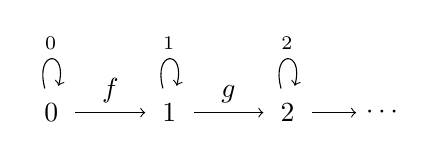
\begin{tikzpicture}[
]
% Objects (circles)
\node[minimum size=0.6cm] (o1) at (0,-1) {0};
\node[minimum size=0.6cm] (o2) at (1.5,-1) {1};
\node[minimum size=0.6cm] (o3) at (3,-1) {2};
\node (dots) at (4.2,-1) {$\cdots$};

% Arrows between objects
\draw[->] (o1) -- node[above] {$f$} (o2);
\draw[->] (o2) -- node[above] {$g$} (o3);
\draw[->] (o3) -- (dots);

\draw[->] (o1) edge[loop above] node[above] {$\id_0$} (o1);
\draw[->] (o2) edge[loop above] node[above] {$\id_1$} (o2);
\draw[->] (o3) edge[loop above] node[above] {$\id_2$} (o3);
\end{tikzpicture}
\end{center}

Given a category $\calC$, a $\calC$-indexed set associates each object of
a category with a set. 
Let's consider a concrete $\calC$-indexed set called $F$.
We can draw $F$ as a ``balloon picture'' like this:

\begin{center}
  \includegraphics[width=175px]{fig/balloon-1.png}
\end{center}

Above each object is drawn a (in this case, finite) set. 
$F_1$ is the set $\{a, b, c\}$, and $F_2$ is is the set 
$\{d, e\}$. 
In addition to associating each object with a set, 
a $\calC$-indexed set also associates each morphism $X \mor{f} Y$
with a function $F_Y \to F_X$, which we can draw on the balloon 
picture like so:

\begin{center}
\includegraphics[width=175px]{fig/balloon-2.png}
\end{center}

Intuitively, we can see that $F$ is describing a relation between two 
categories: our category of interest $\calC$, and an ``external''
category of sets and functions. This relation is called a \textbf{functor}.
Functors have actions on objects 

% \begin{tikzpicture}[
%   node distance=1.5cm,
%   morphism/.style={-Stealth, thick}
% ]

% % Top row of labels
% \node (v) at (0,2) {$v$};
% \node (c) at (3,2) {$c$};

% % Middle row
% \node (y) at (-1.5,1) {$y$};
% \node (w) at (0,1) {$w$};
% \node (a) at (3,1) {$a$};

% % Bottom row (just above the objects)
% \node (x) at (-1.5,0) {$x$};
% \node (h) at (0,0) {$h$};
% \node (b) at (3,0) {$b$};

% % Objects (circles)
% \node[circle, draw, minimum size=0.6cm] (o1) at (0,-1) {0};
% \node[circle, draw, minimum size=0.6cm] (o2) at (1.5,-1) {1};
% \node[circle, draw, minimum size=0.6cm] (o3) at (3,-1) {2};
% \node (dots) at (4.2,-1) {$\cdots$};

% % Arrows between objects
% \draw[morphism] (o1) -- (o2);
% \draw[morphism] (o2) -- (o3);
% \draw[morphism] (o3) -- (dots);

% \end{tikzpicture}




% \begin{center}
%  \begin{tikzpicture}[]

% % Objects
% \node (A) at (0,0) {$A$};
% \node (B) at (3,0) {$B$};
% \node (C) at (1.5,2.5) {$C$};

% % Identity morphisms (loops)
% \draw[->] (A) edge[loop left] node[left] {$\text{id}_A$} (A);
% \draw[->] (B) edge[loop right] node[right] {$\text{id}_B$} (B);
% \draw[->] (C) edge[loop above] node[above] {$\text{id}_C$} (C);

% % Morphisms between objects
% \draw[->] (A) -- node[below] {$f$} (B);
% \draw[->] (A) -- node[left] {$g$} (C);
% \draw[->] (C) -- node[right] {$h$} (B);
% \node[draw, fit=(A)(B)(C), inner sep=1cm, rectangle] {};
% \end{tikzpicture}
% \end{center}


Throughout this section we will work with an arbitrary category \(\calC\).

\begin{definition}[$\calC$-indexed set]
  A $\calC$-indexed set is a functor $F : \calC^\text{op} \Rightarrow \Set$.
\end{definition}

\begin{example}
  Recall that \(\mathsf{STLC}\) is a category
  whose objects are types and whose morphisms \(A \to B\)
  are terms \(x : A \vdash M : B\) quotiented by \(\beta\eta\)-equivalence.
  For each type \(A\),
  the following defines a \(\mathsf{STLC}\)-indexed set \(\mathsf{Tm}(A)\):
  \begin{align}
  \mathsf{Tm}(B)(A) &= \text{the set of morphisms \(A\to B\)} \\
  \mathsf{Tm}(B)(N : A'\to A)
  &= (x\ofty A \vdash M : B) \mapsto (x'\ofty A' \vdash M[N/x] : B)
  \end{align}
\end{example}
This example is a special case of a canonical kind of \(\calC\)-indexed set.
\begin{definition}
  The \emph{representable \(\calC\)-indexed set at \(X\)}
  is written \(\yo X\) and defined by
  \begin{align}
    (\yo X)(A) &= \text{the set of morphisms \(A \to X\)} \\
    (\yo X)(A)(s : A' \to A) &= (f : A \to X) \mapsto (f \circ s : A' \to X)
  \end{align}
\end{definition}

\begin{definition}
  \sloppy
  Let \(P\) and \(Q\) be \(\calC\)-indexed sets.
  A \emph{\(\calC\)-indexed function}
  from \(P\) to \(Q\),
  written \(\alpha : P \Rightarrow Q\),
  is a family of functions \(\alpha_X : PX \to QX\)
  that ``respects substitution''
  in the sense that \(\alpha_{X'}(x\cdot_P p) = \alpha_X(x)\cdot_p p\).
\end{definition}

\begin{itemize}
\item \(\calC\)-indexed functions can be composed:
  the composition of \(\alpha : Q \Rightarrow R\)
  and \(\beta: P \Rightarrow Q\),
  written \(\alpha\circ\beta : P \Rightarrow R\),
  is defined by \((\alpha\circ\beta)_X = \alpha_X \circ \beta_X\).
\item For each \(\calC\)-indexed set \(P\),
  there is a \(\calC\)-indexed function \(\idt_P : P \Rightarrow P\)
  defined by \(\idt_{P,X} = \left(PX \xrightarrow{\idt_{PX}} PX\right)\).
\end{itemize}
By now you may have noticed that \(\calC\)-indexed sets and functions
look like they ought to form a category. More on this later.

\begin{definition}
  Two \(\calC\)-indexed sets \(P,Q\)
  are \emph{isomorphic}
if there are \(\calC\)-indexed functions \(\alpha : P \Rightarrow Q\)
and \(\beta : Q \Rightarrow P\)
such that \(\alpha\circ\beta=\idt_Q\) and \(\beta\circ\alpha=\idt_P\).
\end{definition}

\begin{definition}
  A \(\calC\)-indexed set \(P\) is \emph{representable}
  if there is an isomorphism \(\alpha : P \cong \yo X : \beta\)
  for some object \(X\) of \(\calC\).
\end{definition}


\chapter{Yoneda III: universal constructions, elements, and properties}

\begin{definition}
  \sloppy
  Given two \(\calC\)-indexed sets \(P\) and \(Q\),
  their \emph{product} \(P\times Q\)
  is the \(\calC\)-indexed set defined by
  \((P\times Q)(X) = P(X)\times Q(X)\),
  with substitution defined by
  \((x,y)\cdot_{P\times Q} p = (x\cdot_P p, y\cdot_Q p)\).
\end{definition}

\begin{proposition}
  Let \(X\) and \(Y\) be two objects of a category \(\calC\).
  An object \(P\) is a product of \(X\) and \(Y\)
  if and only if \(\yo P\) is isomorphic to \(\yo X \times \yo Y\).
\end{proposition}

\begin{definition}
  Given two objects \(X\) and \(Y\) of a category \(\calC\),
  there is a \(\calC\)-indexed set of \emph{closures},
  written \(\mathsf{Clos}(X,Y)\),
  defined by \(\mathsf{Clos}(X,Y)(\Gamma) = \calC(\Gamma\times X, Y)\),
  with substitution defined by
  \[
    \mathsf{Clos}(X,Y)(s : \Gamma'\to \Gamma)(f : \Gamma\times X \to Y)
    = \angled{\gamma',x} \mapsto f \circ \angled{s\circ \gamma', x}
  \]
  on generalized elements.
\end{definition}

\begin{proposition}
  Let \(X\) and \(Y\) be two objects of a category \(\calC\).
  An object \(E\) is the exponential \(Y^X\)
  if and only if \(\yo E\) is isomorphic to \(\mathsf{Clos}(X,Y)\).
\end{proposition}

\begin{proposition}
  Suppose the \(\calC\)-indexed set \(P\) is represented
  by the object \(X\).
  Then there exists an element \(u \in PX\),
  called the \emph{\(P\)-universal element},
  which satisfies the following \emph{universal property}:
  for any object \(\Gamma\) and any element \(g \in P\Gamma\),
  there exists a unique morphism \(\hat g : \Gamma \to X\)
  such that \(g = u \cdot_P \hat g\).
\end{proposition}

\begin{itemize}
\item In the case of the product, with \(\yo P \cong \yo X \times \yo Y\),
  the universal element is an element \(u \in \calC(P,X) \times \calC(P,Y)\),
  which is a pair of morphisms \(P\to X, P\to Y\).
  The universal property of this pair is that any other pair \(\Gamma \to X,\Gamma\to Y\)
  factors uniquely through it---precisely the universal property of products
\item In the case of exponents, with \(\yo E \cong \calC(A\times(-),B)\),
  the universal element is an element \(u \in \calC(A \times E,B)\),
  which is a morphism \(A \times E \to B\).
  The universal property of this morphism is that any other morphism
  \(A \times \Gamma \to B\)
  factors uniquely through it---precisely the universal property of exponents.
\end{itemize}

\chapter{Yoneda IV}

%% - Grothendieck universes
%% - The category Set
%% - Functors; opposite categories; C-indexed sets as functors
%% - Natural transformations; C-indexed functions as natural transformations
%% - The Yoneda lemma (without showing naturality in P,c)

%% \begin{itemize}
%% \item Functors form a category where morphisms are natural transformations \begin{itemize}
%%     \item Natural transformations as homotopies between diagrams
%%       (the \(C\to D^\to\) example revisited)
%%     \item Natural transformations as polymorphic maps
%%   \end{itemize}
%% \item Definition of Yoneda embedding
%% \item Restatement of universal properties from previous week in terms of Yoneda embedding
%% (e.g., for products, \(\yo(a\times b) \cong \yo(a)\times \yo(b)\).)
%% \item Yoneda embedding full and faithful. Use this to quickly prove some basic facts:
%%   associativity and commutativity of sums and products, distributivity of products over sums,
%%   ...
%%   These imply type isomorphisms in STLC and Set, entailments of propositional logic.
%% \item Yoneda preserves limits.
%%   This gives a quick proof that all limits can be constructed from products and equalizers.
%%   From this we can compute limits in STLC (it won't have all of them
%%   but it will have some).
%% \end{itemize}

%% \todo: \begin{itemize}
%% \item Slice over c is category of elements of yo c
%% \end{itemize}
